%%this is ci2014/book/local_topology.tex
Visualization tools often decompose data into structure and
attributes~\cite{vtk}. Due to the discrete nature of digital
computers, any numerical function to be visualized must be sampled and
measured at a discrete set of points. However, rendering a
visualization typically requires knowledge of the values between the
samples to produce a perceptually continuous image from arbitrary
viewpoints. Structure encapsulates both the locations and connectivity
relations onto which attributes are superimposed. Structural locations
specify the locations of sampled measurements while connectivity
constrains the interpolation problem. Note that some authors further
decompose structure further into topology and geometry~\cite{weiler},
however, in the context of this research, topology is synonymous with
the structure abstraction.

\sciwms{} adopts the \cfugrid{} conventions for defining a topology. A
topology is always embedded in either $\mathbb{R}^1$, $\mathbb{R}^2$
or, $\mathbb{R}^3$ while the dimension of a topology encapsulates the
connectivity of coordinate locations within the ambient space. For example, a
topology with dimension 0 is a set of disconnected points, a 1D
topology consists of lines or curved boundaries, a 2D topology is a
set of planes or surfaces enclosed by a set of edges
(e.g. triangulation's) and a 3D topology specifies a volume enclosed
by a set of faces.

Attributes are defined as numerical quantities that are associated
with the topology. For example, an atmospheric model may estimate wind
direction at the points of a 2D topology while other may specify air
temperature at the centroid of each volume specified by a 3D
topology. Attributes may also have their own dimensionallity. An
attribute specifying temperature or sea-surface-height are scalars
while wind directions are vector valued, tensor valued attributes are
also possible.

\subsection{Local Topology Cache}
\begin{figure}[ht!]
  \centering
  \begin{subfigure}[t]{0.45\textwidth}
    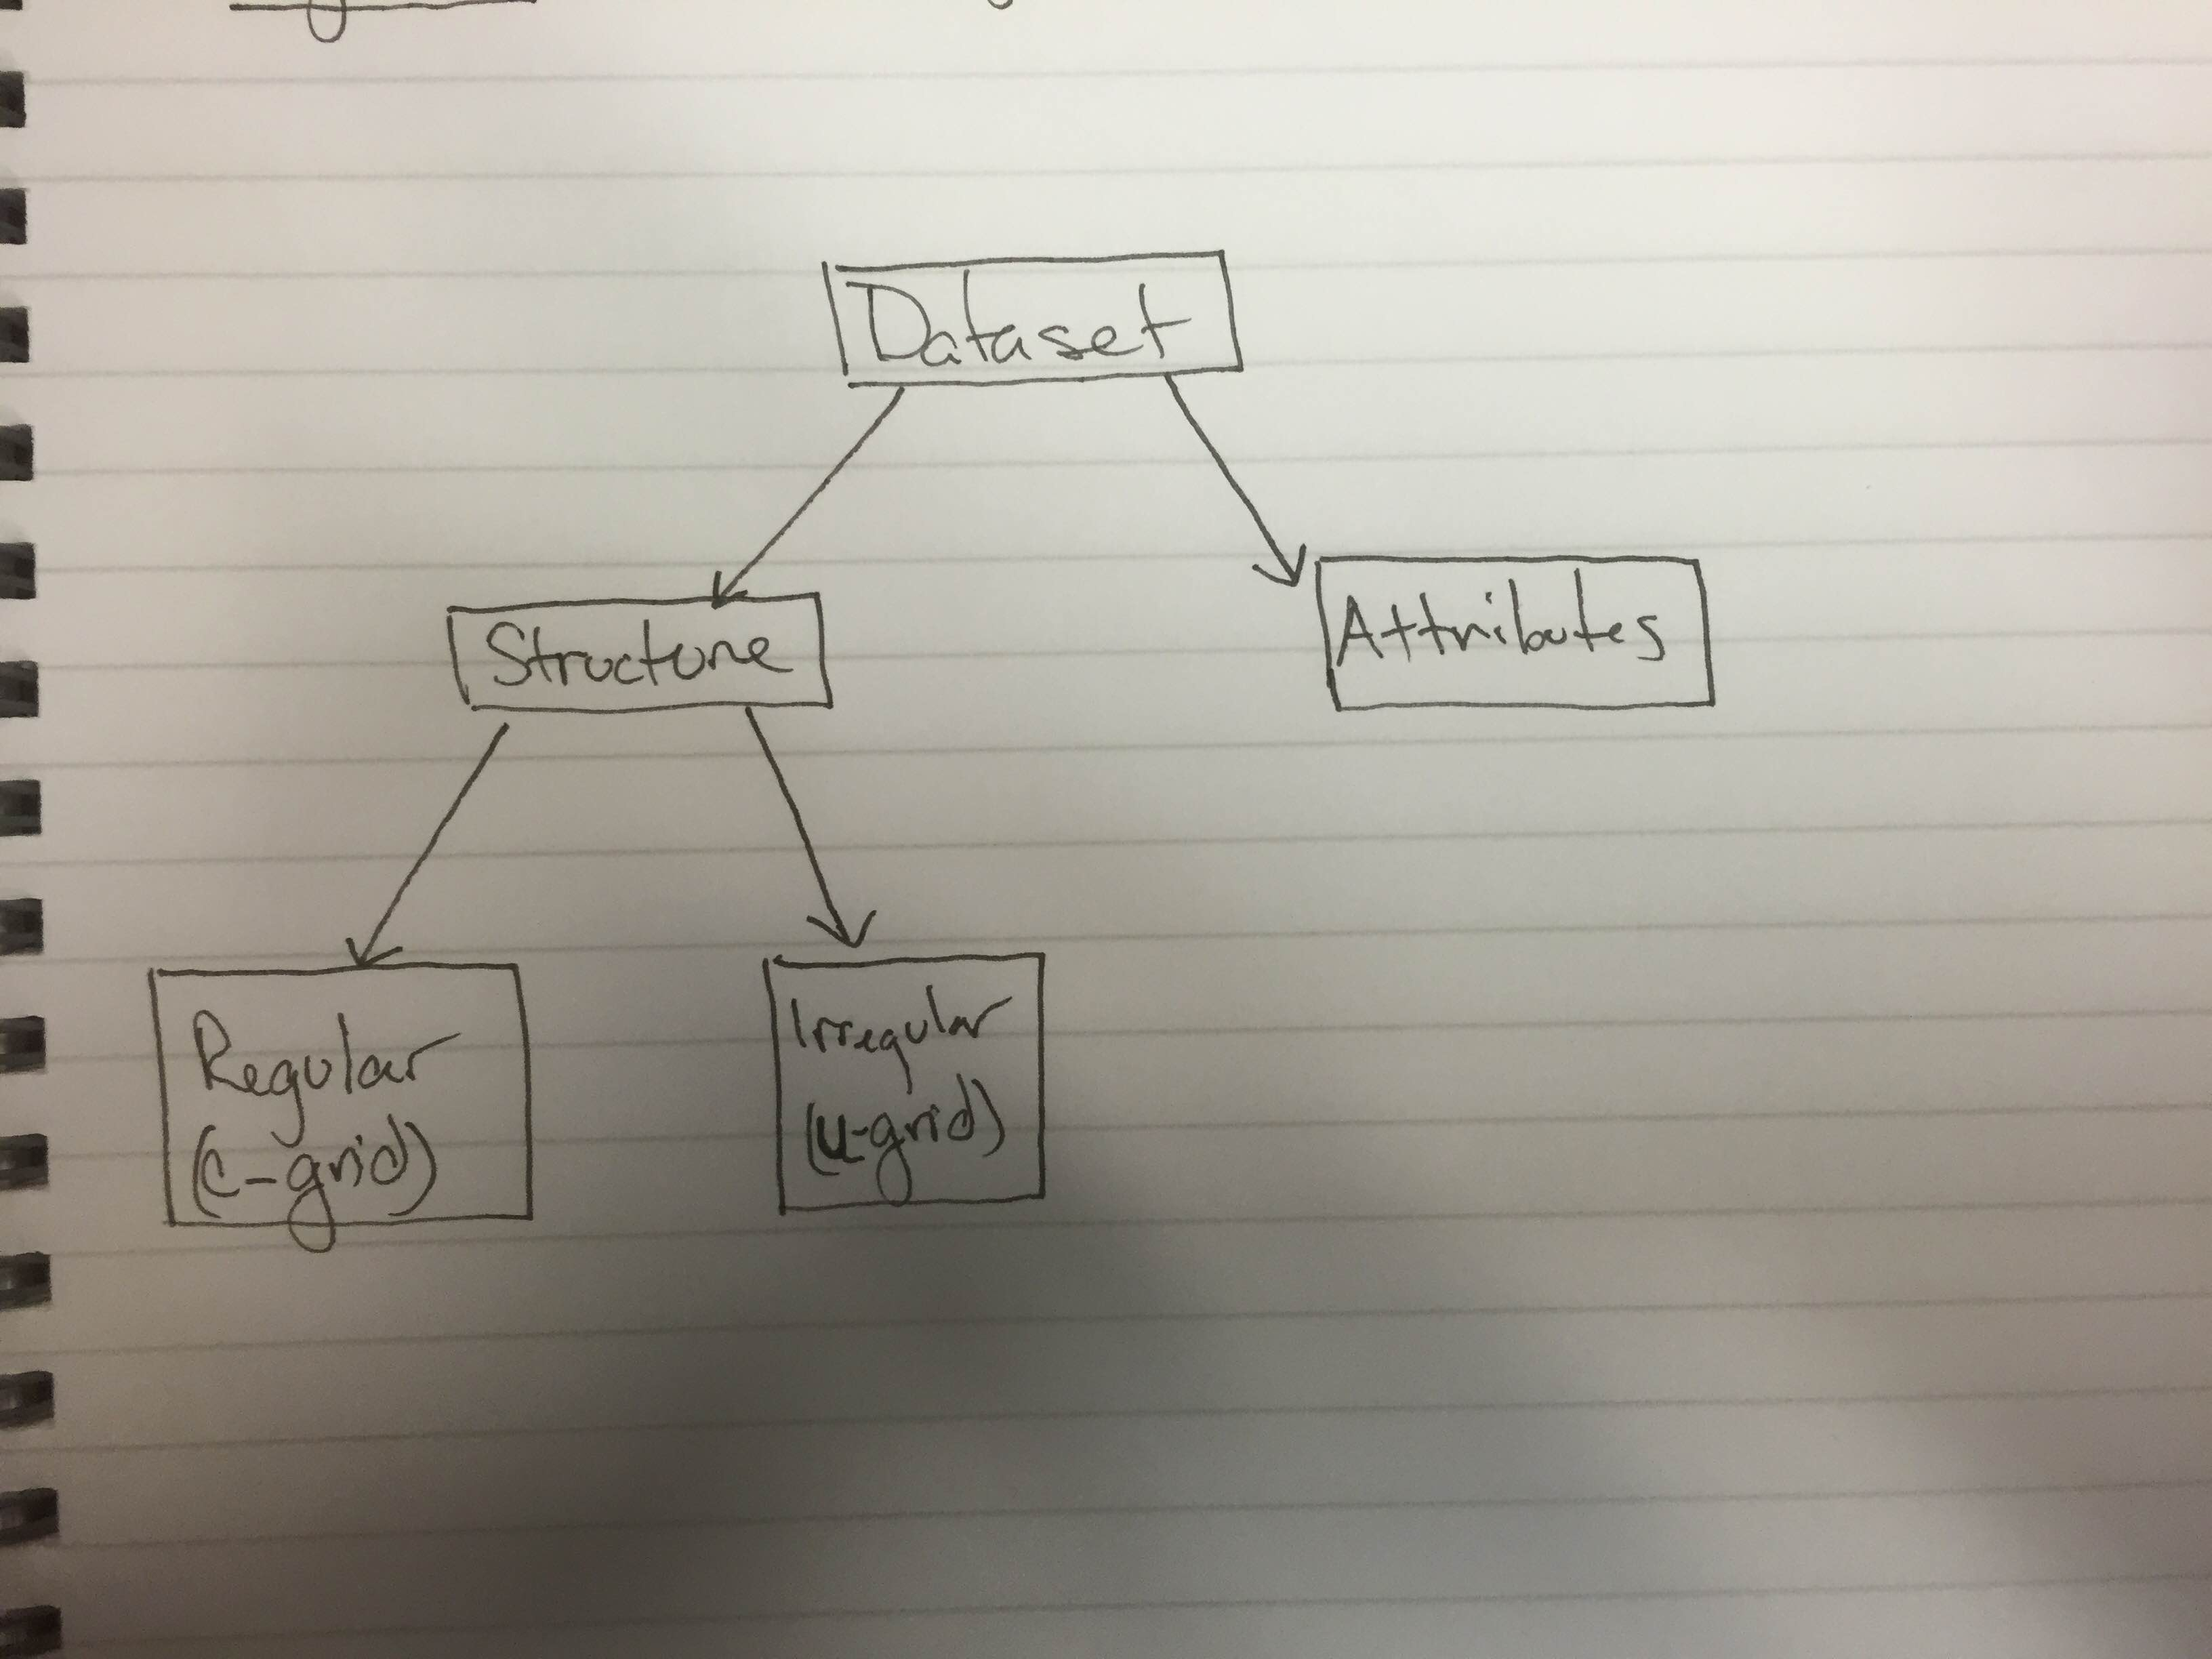
\includegraphics[width=\textwidth]{../figs/data_hierarchy_rough}
  \end{subfigure}
\end{figure}

\subsection{Topology Types}
Topologies are further classified as either regular or irregular or
{\bf \cgrid{}} and {\bf \ugrid} in \sciwms{} terminology.
\paragraph{{\bf \cgrid{}} topologies refer geo-referenced locations and geometries that can be analytically specified, e.g., rectilinear
or curvilinear grids. Storing \cgrid{} topologies amount to storing
the closed form formula. Algorithms for processing \cgrid{}s such as
finding nearest neighbors or finding points that fall withing a
polygonal subset are computed directly using the implicit \cgrid{}
representation.}

\paragraph{{\bf \ugrid{}} are defined as topologies that are not regular, i.e. do not admit a closed form representaqtion. \ugrid{} topologies typically require a definition via explicit enumeration, requiring spatially-aware data structures for optimal storage and processing.}

Following these conventions, \sciwms{} decomposes an externally hosted
dataset into a structure (topology), defined as a geo-referenced
spatial set of locations and connections, and the underlying data
attribute layer.

For example, atmospheric and oceanagrphic models typically define a
fixed topology covering a particular spatial extent of the earth. A
model will extimate attributes of interest such as sea-surface-height,
wind or current magnitudes and directions. The topology of the model
referrs to positions and connectivity of the locations for which
attributes are to be computed. While a model produces data associated
with every location specified by the topology, visualizations are
typically generated for a subset of the topology (a region of
interest) and a single attribute such as current direction. It is
therefore paramount to the efficiency of visualization software to
represent topologies in such a way as to optimize topology storage and
reduction to facilitate efficient attribute retrieval. 

To this end, when an dataset endpoint is submitted to \sciwms{}, the
topology of the underlying endpoint is stored locally to \sciwms{} and
a database of topology-endpoint associations are maintained as
visualized in Figure~\ref{fig:sciwms_topology_endpoints}. 

\begin{figure}[ht!]
  \centering
  \begin{subfigure}[t]{0.45\textwidth}
    \includegraphics[width=\textwidth]{../figs/topology_mem_model}
  \end{subfigure}
  \begin{subfigure}[t]{0.455\textwidth}
    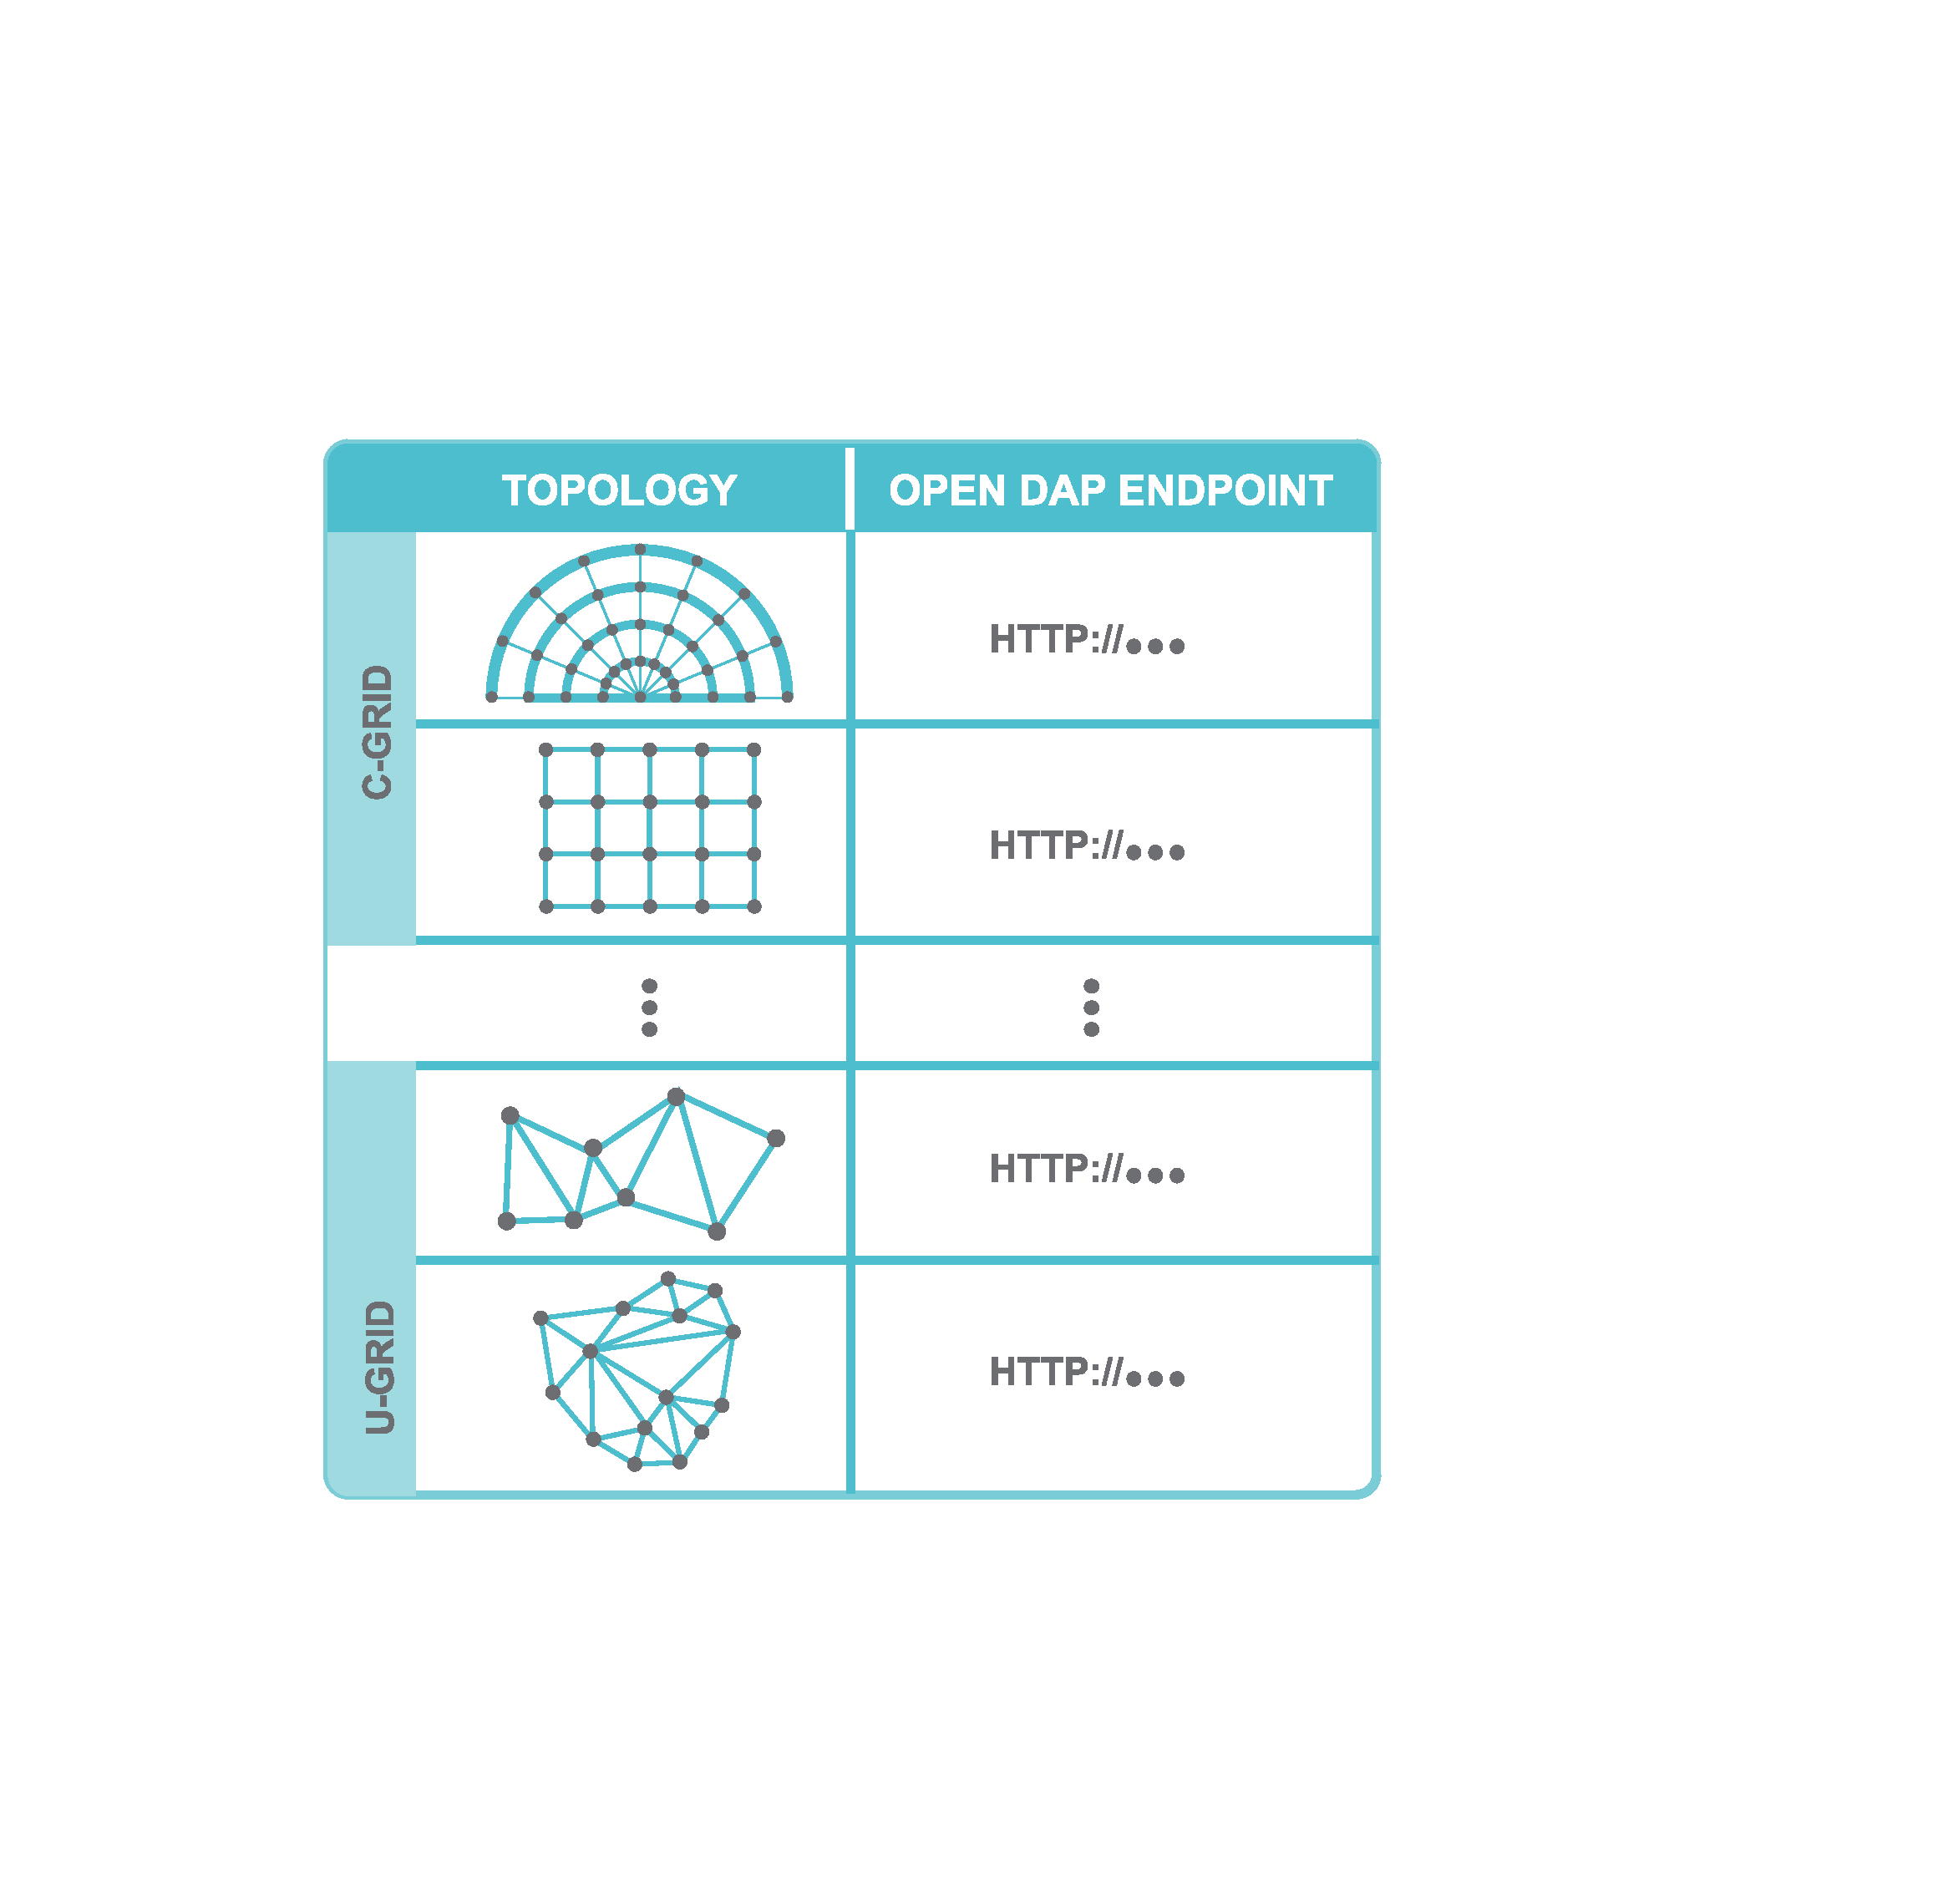
\includegraphics[width=\textwidth]{../figs/sciwms_book_db_topology_endpoints.pdf}
    \caption{\Sciwms{} topology and endpoint data store.}
    \label{fig:sciwms_topology_endpoints}
  \end{subfigure}
\end{figure}


